\begin{enumerate}
\item Ответ: можно. Одно из возможных решений:

\begin{center}
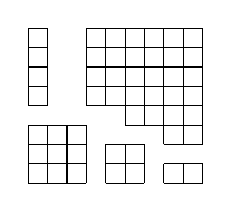
\begin{tikzpicture}[x=7,y=7]
\draw[step=1] (0,0) grid (3, 3);
\draw[step=1] (4,0) grid (6, 2);
\draw[step=1] (7,0) grid (9, 1);
\draw[step=1] (0,4) grid (1, 8);

\draw[step=1] (3,4) grid (9, 8);
\draw[step=1] (5,3) grid (9, 4);
\draw[step=1] (7,2) grid (9, 3);
\end{tikzpicture}
\end{center}

\item Ответ: 0. Прибавив к первой строке все остальные, получим нулевую строку, так как по теореме Виета сумма корней равна нулю.

\item Докажем, что касательные к параболе, проведенные из любой точки на директрисе параболы, --- взаимно перпендикулярны.

$F$ --- фокус, $d$ --- директриса, $AB$ --- хорда параболы, проходящая через фокус $F$, $A_1$, $B_1$ --- проекции $A$, $B$ на $d$. 

\begin{center}
%\input{solution/pictures/2013-2014-3}
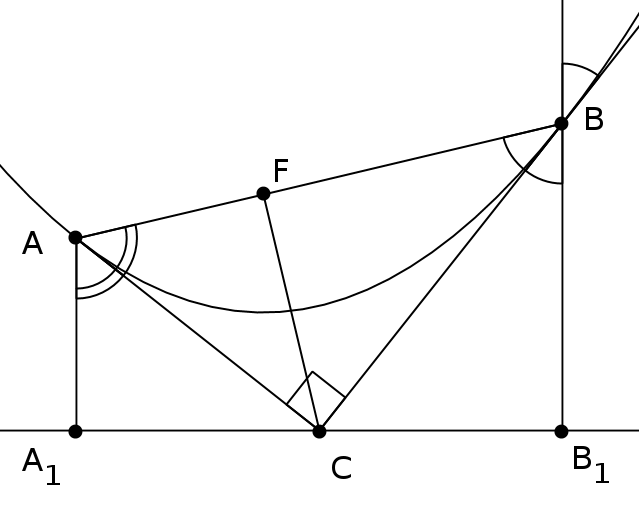
\includegraphics{solution/pictures/2013-2014-3}
\end{center}

Свойство 1. Касательные к параболе, проведенные в концах хорды $AB$, взаимно перпендикулярны. Утверждение легко получить с учетом того, что прямые $AA_1$ и $BB_1$ параллельны, а $AC$ и $BC$ --- биссектрисы углов $\angle ABB_1$ и $\angle BAA_1$ (согласно оптическому свойству).

Свойство 2. $C$ --- точка пересечения касательных --- лежит на директрисе. В силу равенства треугольников $\Delta AA_1C$ и $\Delta AFC$, $\Delta BB_1C$ и $\Delta BFC$, получаем $\angle A_1CB_1 = \pi$.

\begin{comment}
$F$ --- фокус. $O$ --- вершина. $d$ --- директриса. $l$ --- касательная в точке $O$. $A$ и $B$ --- точки касания. $A_1$ и $B_1$ --- их проекции на $l$. $A_2$ и $B_2$ --- точки пересечения касательных с $l$. $A_3$ и $B_3$ --- проекции на $d$.

Свойство 1. Касательная в точке $B$ делит отрезок $OB_1$ пополам. По определению параболы $FB = BB_3$. Согласно оптическому свойству касательная является биссектрисой угла $FBB_3$, значит середина $FB_3$ лежит на касательной из $B$. По определению параболы $FO = B_1B_3$, то есть середина $FB_3$ есть и середина $OB_1$.
\end{comment}

\item Последовательно полагайте в исходном соотношении:
\begin{enumerate}
\item $a = x$, $b = 0$, $c = 0$;
\item $a = x * 0$, $b = 0$, $c = y$;
\item $a = 0$, $b = x$, $c = 0$;
\item $a = 0 * x$, $b = 0$, $c = y$.
\end{enumerate}

\item а) Количество интересных перестановок порядка $N$ вычисляется с помощью формулы включения-исключения:
$$S(N) = N!-{\frac {N!}{1!}}+{\frac {N!}{2!}}-{\frac {N!}{3!}} + \dots +(-1)^{N}{\frac {N!}{N!}}=\sum _{k=0}^{N}(-1)^{k}{\frac {N!}{k!}}
$$

б) $e^{-1}$.

\item Ответ: $k = 2$. Замена: $t = \ln{x}$. Тогда
$$\int\limits_{1}^{2} \left( 1 + k \ln{x} \right) x^{x^k + k - 1} dx = \int\limits_{0}^{\ln{2}} \left(e^{te^{kt}} \right)' dt = $$
$$=\left. e^{te^{kt}} \right|_{0}^{\ln{2}} = 2^{2^k} - 1.$$

\item a) Для любого целого $n$ куб $n$ может давать при делении на 9 только следующие остатки: 0, 1 или 8. Следовательно, числа вида $9k \pm 4$ не могут быть представлены в виде суммы трех кубов.

б) Используйте тождество:
$$6x = (x+1)^3 + (x-1)^3 + (-x)^3 + (-x)^3.$$

\item Ответ: $\frac{(n/2)!}{(n/4)!}$. Из условия следует, что для любого $k$ от 1 до $n$ верно $f(f(k)) = n + 1 - k$, то есть определить $f(f(k))$ можно однозначно. Также очевидно, что $f^4(k) = k$. Из четности $n$ понятно, что $f^2(k) \neq k$. Следовательно, $f(k) \neq k$ и $f^3(k) \neq k$. 

В качестве $f(1)$ можно выбрать любое значение из $n-2$ (кроме 1 и $n$). Сразу однозначно определяются значения $f(1)$, $f(f(1))$ и $f(f(f(1)))$. Далее для $s$ (любых из $n-4$ еще неопределенных значений) можно выбрать любое из $n-6$ допустимых значений (кроме уже определенных 4 значений, $s$ и $n+1-s$). Итог ($n = 4m$):
$$(n-2) \cdot  (n-6) \cdot  ... \cdot  6 \cdot 2 = \frac{(2m)!}{m!}.$$

\item Ответ: $2 - \frac{1}{2^n}$.

Ясно, что многочлен $x P(x) - 1$ имеет степень $n+1$. Его корнями при этом будет $n+1$ число: $2^k$ при $k$ от $0$ до $n$. Значит, этот многочлен представляется в виде 
$$x P(x) - 1 = A (x - 1) (x - 2) ... (x - 2^n).$$
Коэффициент $A$ можно найти, приравнивая свободный член: $A = (-1)^{n+1} \frac{1}{2^{1+2+...+n}}$. Свободный член $P(x)$ равен коэффициенту при $x^1$ в правой части:
$$ - \left(1 + \frac{1}{2} + ... + \frac{1}{2^n} \right).$$

\item Ответ: $\frac{k^2 + k + 2}{2}$. Выберем некоторую вершину $A$: на расстоянии 1 от неё расположено $k$ вершин (обозначим это множество вершин $B$), а на расстоянии 2 ---  $(n - 1 - k)$ вершин (обозначим это множество вершин $C$). Посчитаем количество различных четырехугольников. 

Способ первый: вершины, противоположные $A$ в соответствующем четырехугольнике, обязательно содержатся в $C$. Каждая такая вершина определяет четырехугольник однозначно. Значит, общее количество четырехугольников в графе $\frac{n(n-k-1)}{4}$.

Способ второй: соседи вершины $A$ обязательно содержатся в $B$. Каждая такая пара определяет четырехугольник однозначно. Значит, общее количество четырехугольников в графе $\frac{nk(k-1)}{8}$.

Приравниваем данные соотношения и получаем:
$$n = \frac{k^2 + k + 2}{2}.$$

\end{enumerate}
